%%%%%%%%%%%%%%% Figure from ESA %%%%%%%%%%%%%%%%%%%
% included from otree-graycode.tex
\begin{figure}[H]
    \centering
    \begin{subfigure}{.98\textwidth}
        \captionsetup[subfigure]{justification=centering}
        \begin{subfigure}[t]{.49\textwidth}
            \centering
    	    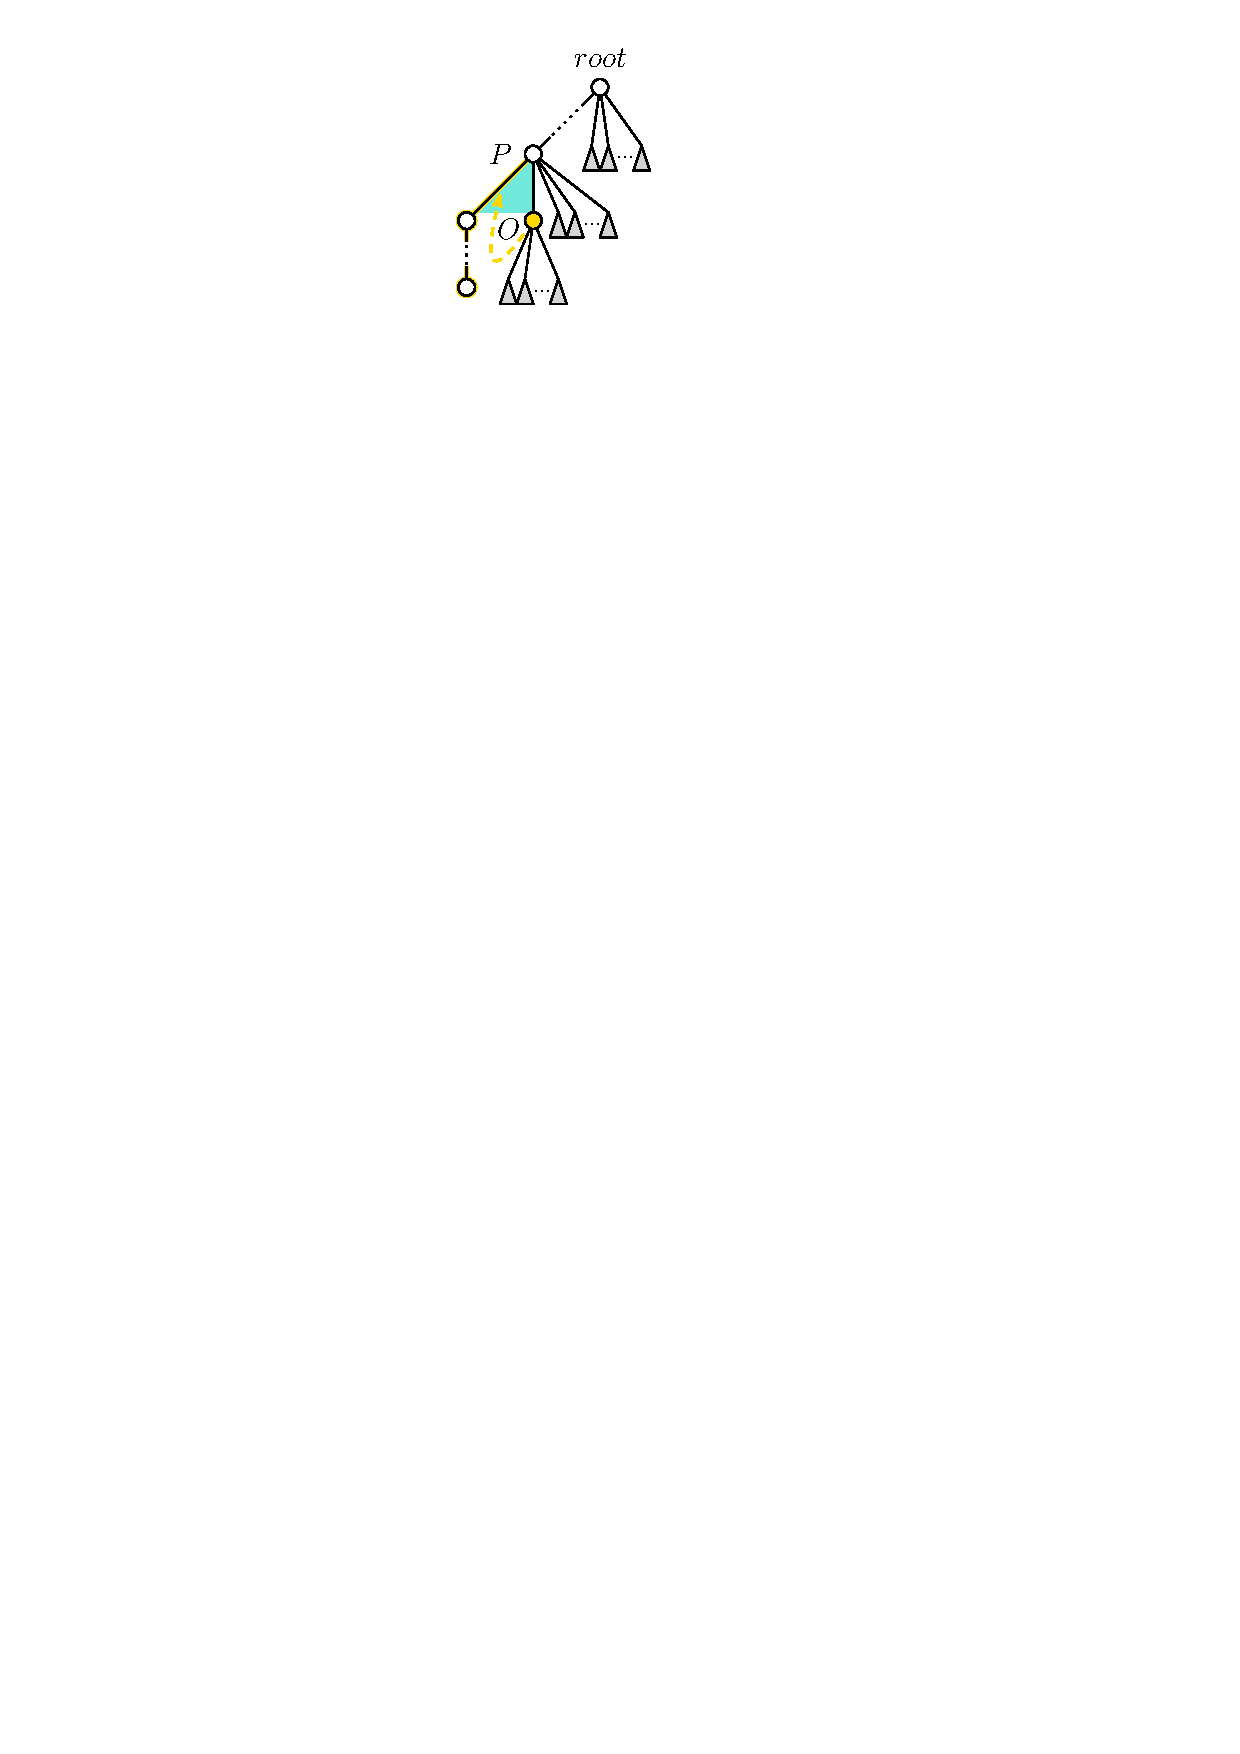
\includegraphics[scale=0.85]{nextTightOr011Before.pdf}
    	    \caption*{Current tree $\tree{T}$ where ${P} = {root}$ or ${O}$ is not a leaf.}
            \label{fig:next1_Before}
        \end{subfigure}
        \hfill
        \begin{subfigure}[t]{.49\textwidth}
    	    \centering
    	    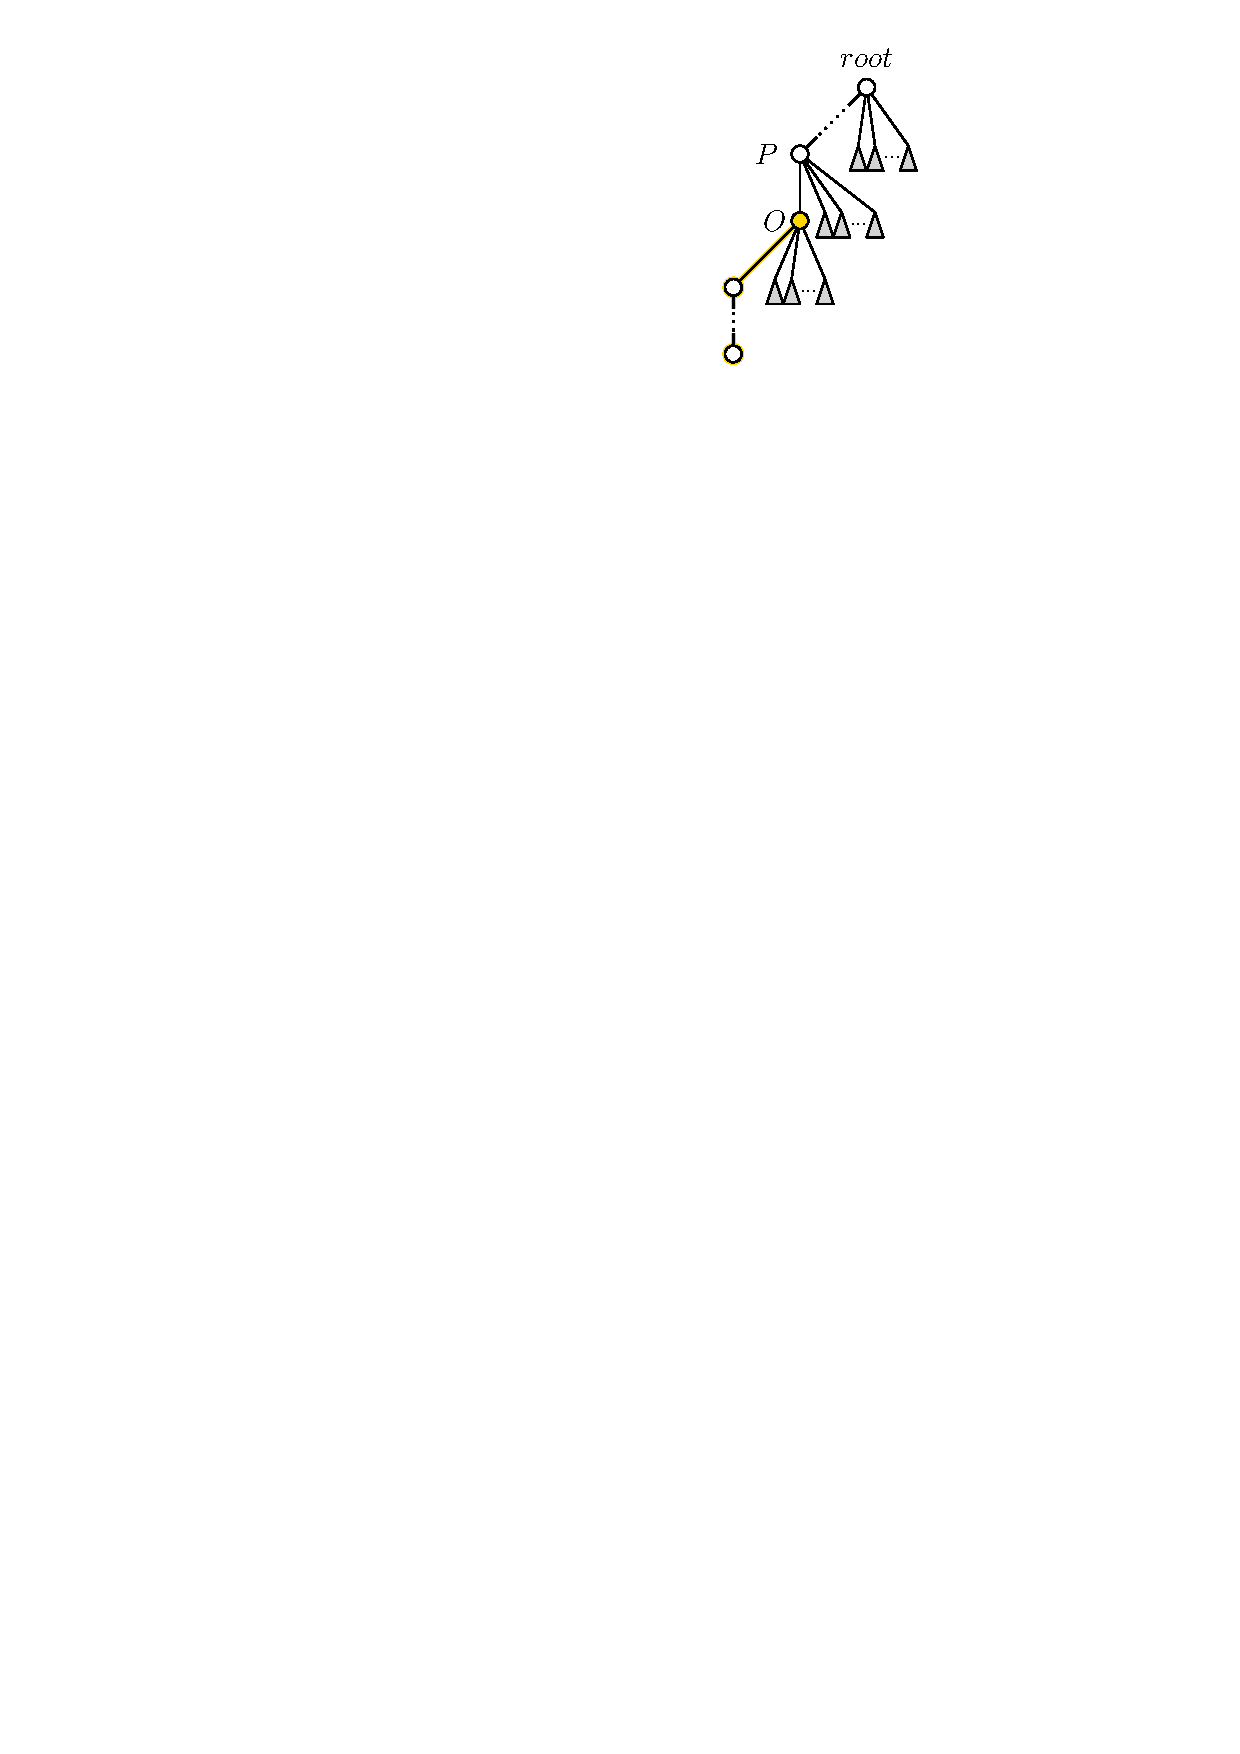
\includegraphics[scale=0.85]{nextTightOr011After.pdf}
    	    \caption*{New tree $\tree{T'}$ is obtained by $\pull[\tree{T}]{{O}}{{P}}$.}
            \label{fig:next1_Intermediate}
        \end{subfigure}
	    \caption{Case \eqref{eq:otree_oneshift}.
	    After the pull, the node ${O}$ is updated to be the new second-child of ${O}$ (if non-null) or the new second-child of ${P}$ (if non-null), or~${null}$.
	    The pull is equivalent to $\pushchild{{O}}{\popchild{{P}}}$.}
        \label{fig:next1}
    \end{subfigure}    

    \vspace{1em}
        
    \begin{subfigure}{.98\textwidth}
        \captionsetup[subfigure]{justification=centering}
        \begin{subfigure}[t]{.32\textwidth}
            \centering
    	    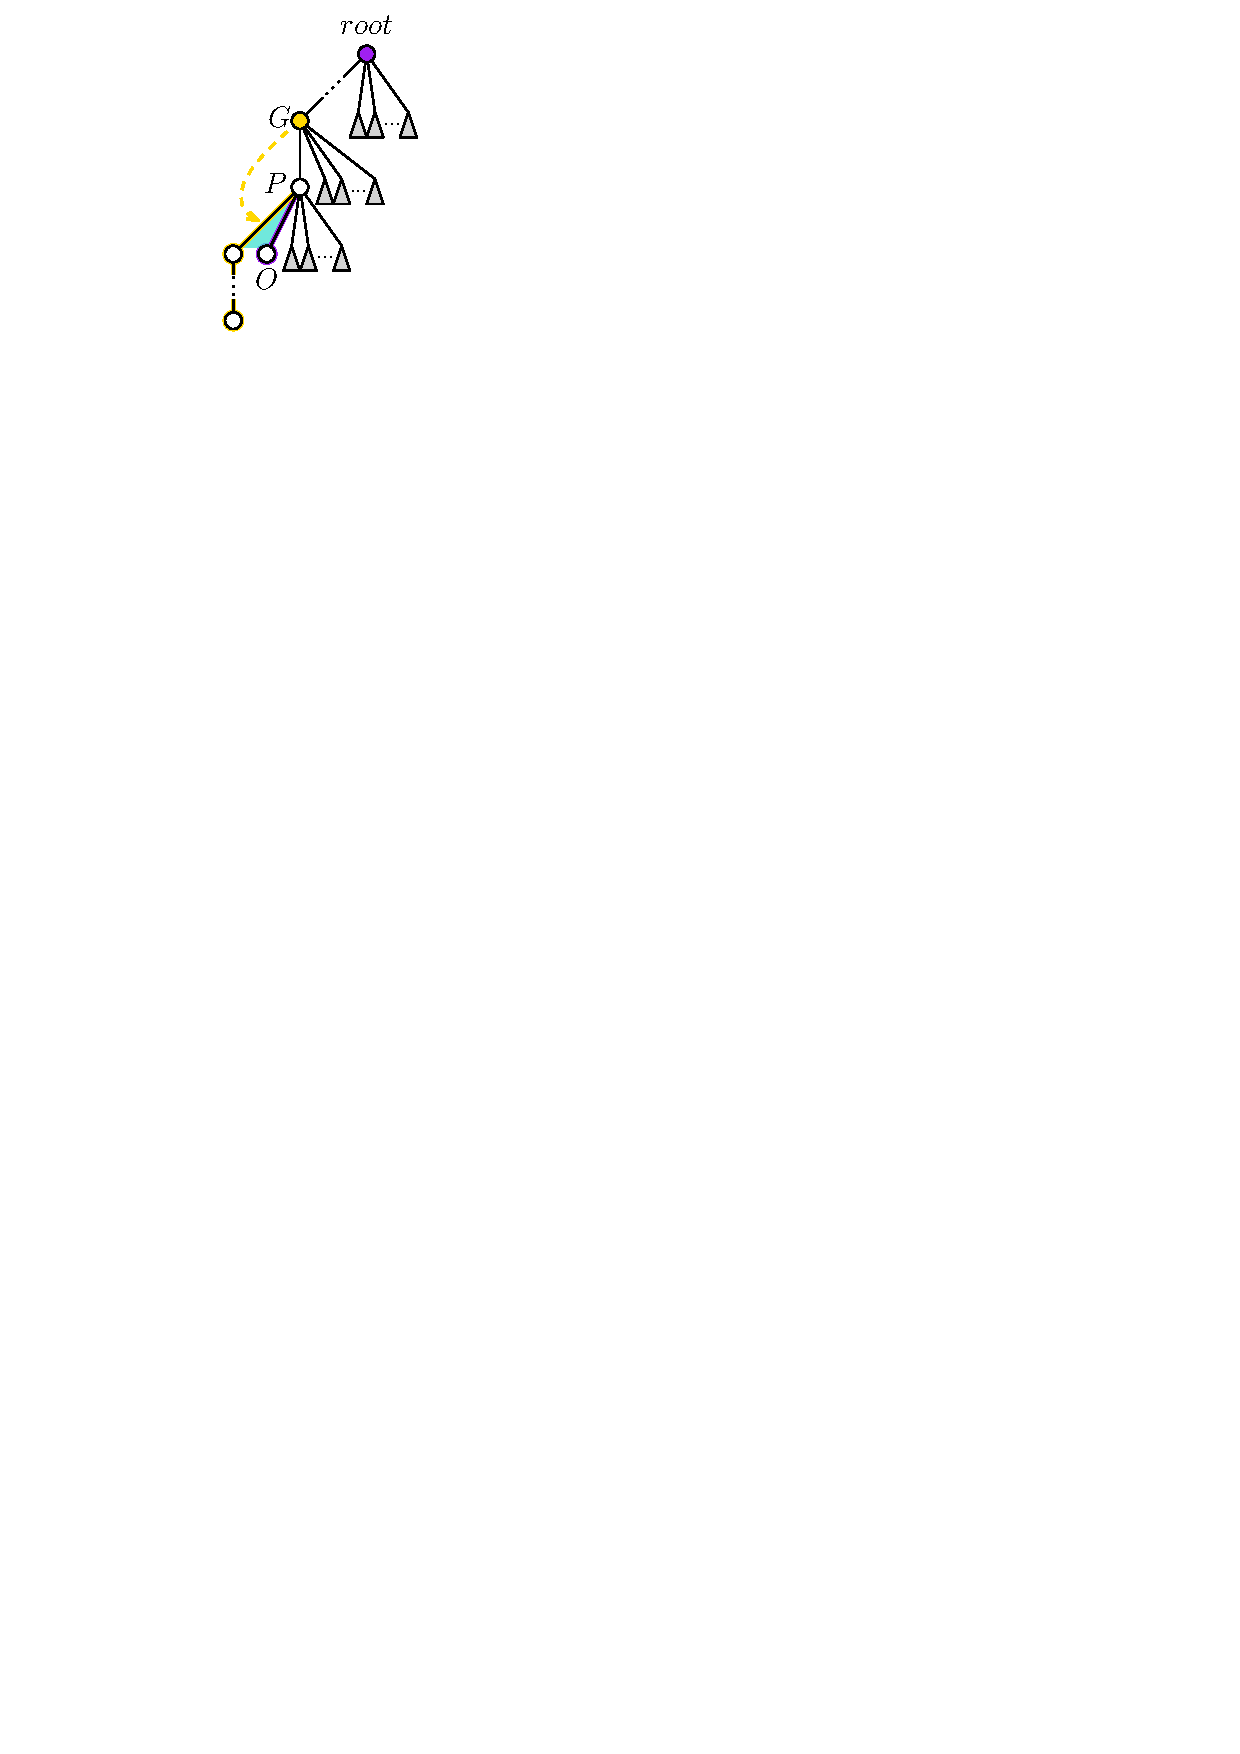
\includegraphics[scale=0.85]{next010Before.pdf}
    	    \caption*{Current tree $\tree{T}$ where ${P} \neq {root}$ and ${O}$ is a leaf.}
            \label{fig:next0_Before}
        \end{subfigure}
        \hfill
        \begin{subfigure}[t]{.32\textwidth}
    	    \centering
    	    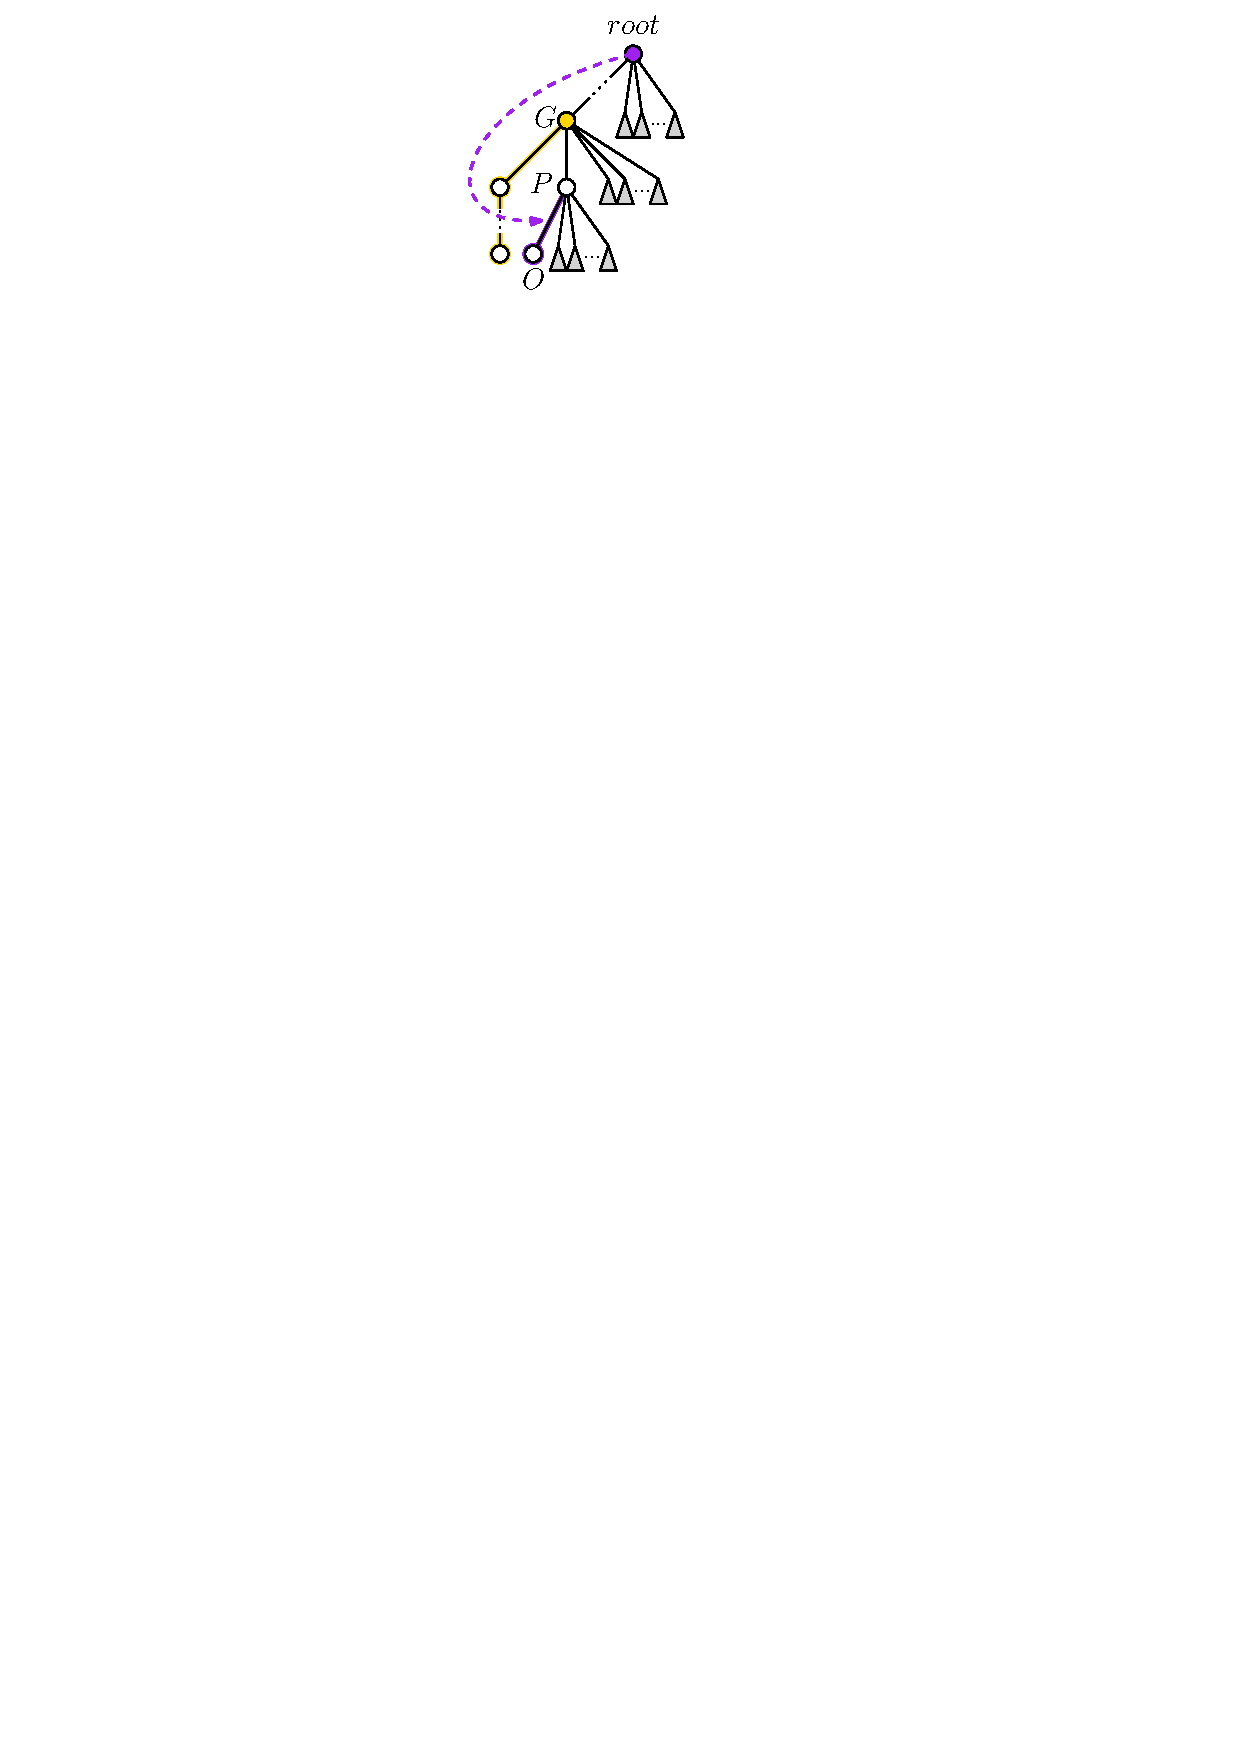
\includegraphics[scale=0.85]{next010Intermediate.pdf}
    	    \caption*{Intermediate tree $\tree{I}$ is obtained by $\pull[\tree{T}]{{G}}{{P}}$.}
            \label{fig:next0_Intermediate}
        \end{subfigure}
        \begin{subfigure}[t]{.32\textwidth}
    	    \centering
    	    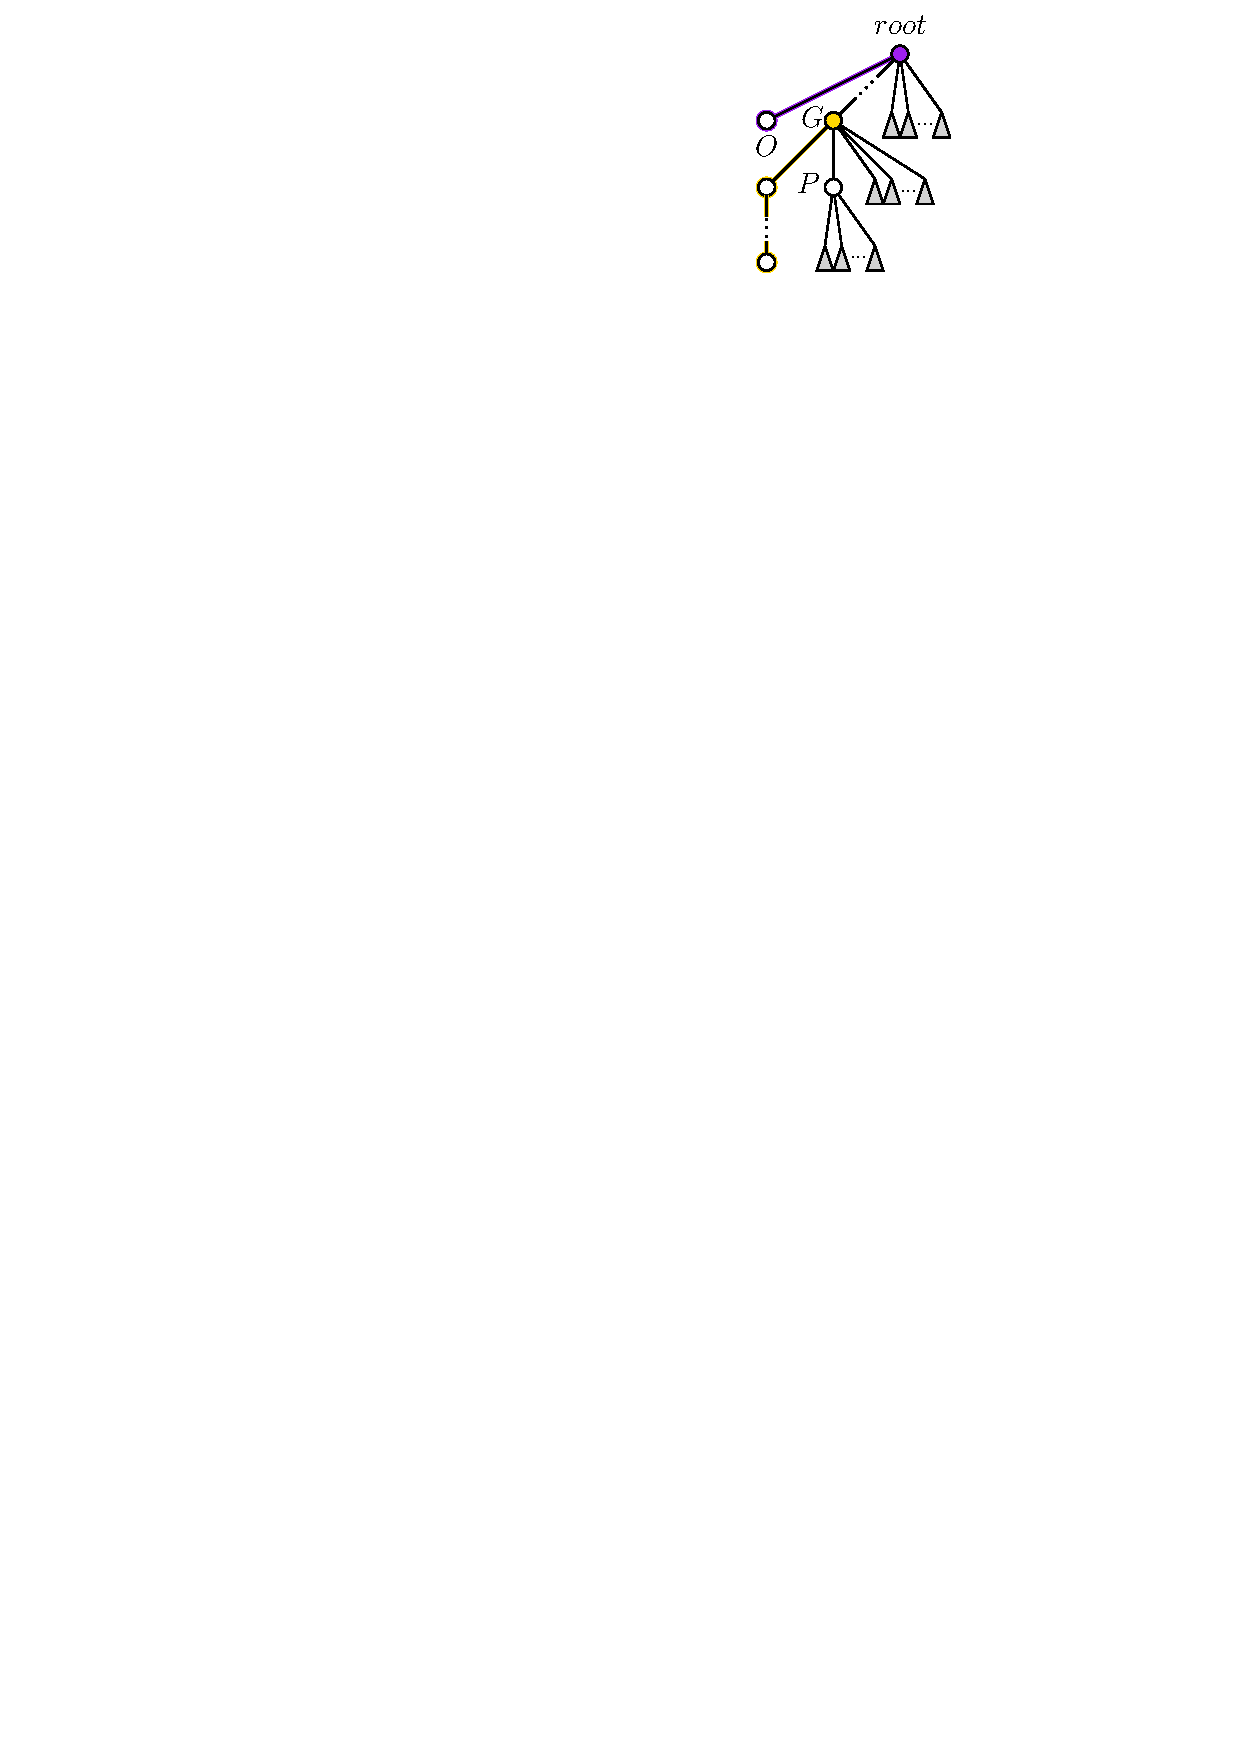
\includegraphics[scale=0.85]{next010After.pdf}
    	    \caption*{New tree $\tree{T'}$ is obtained by $\pull[\tree{I}]{{root}}{{P}}$.}
            \label{fig:next0_After}
        \end{subfigure}
	    \caption{Case \eqref{eq:otree_zeroshift}.
	    After the pull, the node ${O}$ is updated to be the new second-child of ${root}$.
	    The pull operations are equivalent to $\pushchild{{G}}{\popchild{{P}}}$ followed by $\pushchild{{root}}{\popchild{{P}}}$}
        \label{fig:next0}
    \end{subfigure}    
    
    \caption[Our pull Gray code is generated by the two case successor rule in \eqref{eq:otreeRule}.]{Our pull Gray code is generated by the two case successor rule in \eqref{eq:otreeRule}.
    This rule describes how to transform the current ordered tree $\tree{T}$ into the new next ordered tree $\tree{T'}$ using either one or two pulls.
    In these figures, ${O}$ is the first node in a preorder traversal that is not on the path from the root to the leftmost descendent, and ${P}$ is its parent, and ${G}$ is its grandparent (if applicable).
    White circles denote non-null nodes, and grey triangles denote an unspecified number of children and subtrees.
    The pull operations, which are always path-pulls, are highlighted.
    The first pulling node and pulled path are in gold, while the second are in purple.
    The captions also explain how to update the value of ${O}$.}
    \label{fig:next}
\end{figure}

